\documentclass[
a4paper,
17pt,
]{extarticle}

\usepackage{fullpage}
%\usepackage{showframe}

\usepackage[top=2.5cm, bottom=2cm, left=2.4cm, right=2.4cm]{geometry}


\usepackage{moreverb,url}


%--------------------------------------------------------------------
% INPUT, LANGUAGE, TEXT, APPEARANCE, LAYOUT

% hopefully embeds all fonts in pdf
\usepackage[T1]{fontenc}
\usepackage[english]{babel}
\usepackage{pslatex}


%\usepackage[kerning,spacing]{microtype} 
% more compact and arguably nicer
% http://www.khirevich.com/latex/microtype/
\usepackage[
	activate={true,nocompatibility}, % activate={true,nocompatibility} - activate protrusion and expansion
	final, % final - enable microtype; use "draft" to disable
	tracking=true,
	factor=1100, % factor=1100 - add 10% to the protrusion amount (default is 1000)
	stretch=10, % stretch=10, shrink=10 - reduce stretchability/shrinkability (default is 20/20)
	shrink=10]
	{microtype}


% in 2 column layout, make cols in last page equal in size
%\usepackage{flushend}


% Input from relative instead of absolute path
\usepackage{currfile}



%--------------------------------------------------------------------
% GRAPHICS, TIKZ

\usepackage[
dvipsnames,
table,
]{xcolor} % must be early

\usepackage{tikz}
\usetikzlibrary{
arrows,
automata,
calc,
graphs,
graphdrawing,
arrows.meta,
decorations.pathmorphing,
matrix,
positioning,
fit,
}
\usegdlibrary{
layered,
trees,
}

% Allow more options in \includegraphics
\usepackage{graphicx}

\usepackage[space]{grffile} % fix filename space issue

% Include regular tikz image file of a board generated by minotool
\newcommand{\tikzBoard}[1]{%
%\iffalse
\iftrue
	\begin{adjustbox}{scale=0.9}
	\begin{tikzpicture}
	\input{"img/#1.tikz"}
	\end{tikzpicture}
	\end{adjustbox}
\else
	% No more tikz. I'm done with its cosmetic bugs. Just put in raster images instead.
	% Nachteil: Buchstaben in Grafiken sind verpixelt
	\begin{adjustbox}{scale=0.8}
	\includegraphics[]{"img/#1"}
	\end{adjustbox}
\fi
}

% ----------
% latex boxes, nested tikz
% For \xsbox to easily generate saveboxes on the fly
\usepackage{xsavebox}



%--------------------------------------------------------------------
% FRAMED, TABLES, BOXES

\usepackage{framed}
\renewenvironment{leftbar}[1][Gray]%
{%
        \def\FrameCommand%
        {%    
		        {\color{#1}\vrule width 3pt}%
                \hspace{3pt}%
             %\fboxsep=\FrameSep\colorbox{green}%
        }%
        \MakeFramed{\hsize \hsize \advance\hsize-\width\FrameRestore}%
}%
{\endMakeFramed}

\usepackage[most]{tcolorbox}
\tcbset{
frame code={}
center title,
left=0pt,
right=0pt,
top=0pt,
bottom=0pt,
colback=gray!20,
colframe=white,
width=\dimexpr\textwidth\relax,
enlarge left by=0mm,
boxsep=5pt,
arc=0pt,
outer arc=0pt,
}

\usepackage{tabularray}
\UseTblrLibrary{booktabs}

% in the future, just use package tabularray instead
\usepackage{makecell}
\usepackage{nicematrix}

% For \FloatBarrier
\usepackage{placeins}

% For \maxsizebox
\usepackage[export]{adjustbox}

% Control over lists
\usepackage{enumitem}

% Subfigures
\usepackage{subcaption}


%--------------------------------------------------------------------
% MATH, SYMBOLS
\usepackage{amsmath}
\usepackage{amssymb}

% Math: argmin
\DeclareMathOperator*{\argmin}{arg\,min}
\DeclareMathOperator*{\argmax}{arg\,max}



%--------------------------------------------------------------------
% FIGURE CAPTIONS
\usepackage[
%labelfont={it,bf},
%font={sf},
%margin=1.0cm
]{caption}
\captionsetup[figure]{labelformat=empty}


%--------------------------------------------------------------------
%. TODONOTES

% required for multiple optional args
\usepackage{xargs}



%--------------------------------------------------------------------
% BIBLIOGRAPHY, REFERENCES, QUOTES

% enquote*
\usepackage{csquotes}

\usepackage[
colorlinks,
bookmarksopen,
bookmarksnumbered,
hidelinks,
]{hyperref}



% ----------------------------------------------------
% CUSTOM

\usepackage{calc}

% Display of Pentomino strings
\definecolor{strBack}{rgb}{0.90,0.90,0.90}
\newlength{\strWidth}%
\newcommand{\str}[2][strBack]%
{%
\texttt{%
\setlength{\fboxsep}{1pt}%
\settowidth{\strWidth}{#2}%
\colorbox{#1}%
{%
\adjustbox{raise={0pt}{\height}{0pt}}{% Try to ignore depth (e.g. from commas or the letter y).
\parbox[b][1.2pt+\fontcharht\font`X][b]{\strWidth}{\centering#2}%
}}%
}}

% Display of Pentomino pieces
% This uses raisebox twice to counteract that the top of tight frames is closer than the bottom, even if the depth below the baseline is 0. Not sure if the font is messed up or it is just Latex things.
\DeclareRobustCommand*{\FixHeight}{%
    \raisebox{0pt}[\height+0.6pt][0pt]%
}
\newcommand{\piece}[1]%
{%
\protect\textrm{%
\setlength{\fboxsep}{1pt}%
\fbox{%
\FixHeight{#1}%
}%
}%
}

\newcommand*{\strm}{\leavevmode\unskip{\str{+}}\ignorespaces}
\newcommand*{\strs}{\leavevmode\unskip{\str{/}}\ignorespaces}
\newcommand{\strf}{{\str{$\Rightarrow$}}}




% Avoid ripping text apart just to put something at the end of a page
\raggedbottom



%--------------------------------------------------------------------
% DOCUMENT BODY BEGINS
%--------------------------------------------------------------------

\begin{document}

\section{Einführung}

Pentomino ist ein Brettspiel.
Ein Raster aus Zellen muss lückenlos und ohne Überlappung mit Spielsteinen gefüllt werden.
Es gibt 12 Spielsteine, die je genau 5 Zellen bedecken.
Spielsteine dürfen beliebig gedreht und gespiegelt werden.
Derselbe Spielstein darf aber nicht mehrfach benutzt werden.

\begin{figure}[hbt]
\centering

\resizebox{0.99\linewidth}{!}{%
\begin{tabular}{@{}%
c@{\hskip 2pt}%
c@{\hskip 2pt}%
c@{\hskip 2pt}%
c@{\hskip 2pt}%
c@{\hskip 2pt}%
c@{\hskip 1pt}%
c@{\hskip 1pt}%
c@{\hskip 2pt}%
c@{\hskip 2pt}%
c@{\hskip 1pt}%
c@{\hskip 2pt}%
c@{\hskip 2pt}%
@{}}
\adjustbox{scale=0.9}{\tikzBoard{10 intro/Alphabet F}} &
\adjustbox{scale=0.9}{\tikzBoard{10 intro/Alphabet I}} &
\adjustbox{scale=0.9}{\tikzBoard{10 intro/Alphabet L}} &
\adjustbox{scale=0.9}{\tikzBoard{10 intro/Alphabet N}} &
\adjustbox{scale=0.9}{\tikzBoard{10 intro/Alphabet P}} &
\adjustbox{scale=0.9}{\tikzBoard{10 intro/Alphabet T}} &
\adjustbox{scale=0.9}{\tikzBoard{10 intro/Alphabet U}} &
\adjustbox{scale=0.9}{\tikzBoard{10 intro/Alphabet V}} &
\adjustbox{scale=0.9}{\tikzBoard{10 intro/Alphabet W}} &
\adjustbox{scale=0.9}{\tikzBoard{10 intro/Alphabet X}} &
\adjustbox{scale=0.9}{\tikzBoard{10 intro/Alphabet Y}} &
\adjustbox{scale=0.9}{\tikzBoard{10 intro/Alphabet Z}} \\
\piece{F} &
\piece{I} &
\piece{L} &
\piece{N} &
\piece{P} &
\piece{T} &
\piece{U} &
\piece{V} &
\piece{W} &
\piece{X} &
\piece{Y} &
\piece{Z} \\
\end{tabular}%
}

\caption
{
Die zwölf eindeutigen Pentomino-Spielsteine werden meist nach ähnlich aussehenden Buchstaben benannt.
}

\end{figure}


\begin{figure}[hbt]
\centering

\adjustbox{scale=0.90}{\tikzBoard{10 intro/example of closed cell board empty}}
\hspace{0.1\textwidth}
\adjustbox{scale=0.90}{\tikzBoard{10 intro/example of closed cell board solution}}

\caption
{
Ein leeres 6$\times$6-Brett für fünf Spielsteine und seine einzige Lösung mit
% (left to right, then top to bottom)
\rotatebox[origin=c]{-90}{\piece{P}},
\piece{Y},
\rotatebox[origin=c]{180}{\piece{L}},
\piece{N}
und
\rotatebox[origin=c]{-90}{\piece{T}}.
}

\label{fig:example of closed cell board solution}
\end{figure}




\FloatBarrier
\newpage
\section{Lösen mit Spielsteinen}


\FloatBarrier
\subsection{Backtracking}

Die Grundstrategie ist Backtracking:
systematisches Ausprobieren.
Platziere Spielsteine nacheinander.
Probiere jeden Spielstein und jede Ausrichtung.
Wenn nichts passt:
letzte Platzierung zurücknehmen und die nächste Möglichkeit testen.
Weiter so, bis das Brett gefüllt ist oder alle Möglichkeiten erschöpft sind.
(Alle Bretter hier haben genau eine Lösung.)

Das führt sicher zur Lösung, kann aber lange dauern.
Es ist effizienter, zuerst an eingeschränkten Bereichen zu arbeiten:
Je weniger Möglichkeiten an einer Stelle sind, desto wichtiger ist sie.
So lassen sich viele Optionen schnell ausschlie{\ss}en.
Im Idealfall bleibt nur eine Möglichkeit übrig.



\newgeometry{margin=0pt}
%\thispagestyle{empty}
\noindent
\makebox[\paperwidth][c]{%
	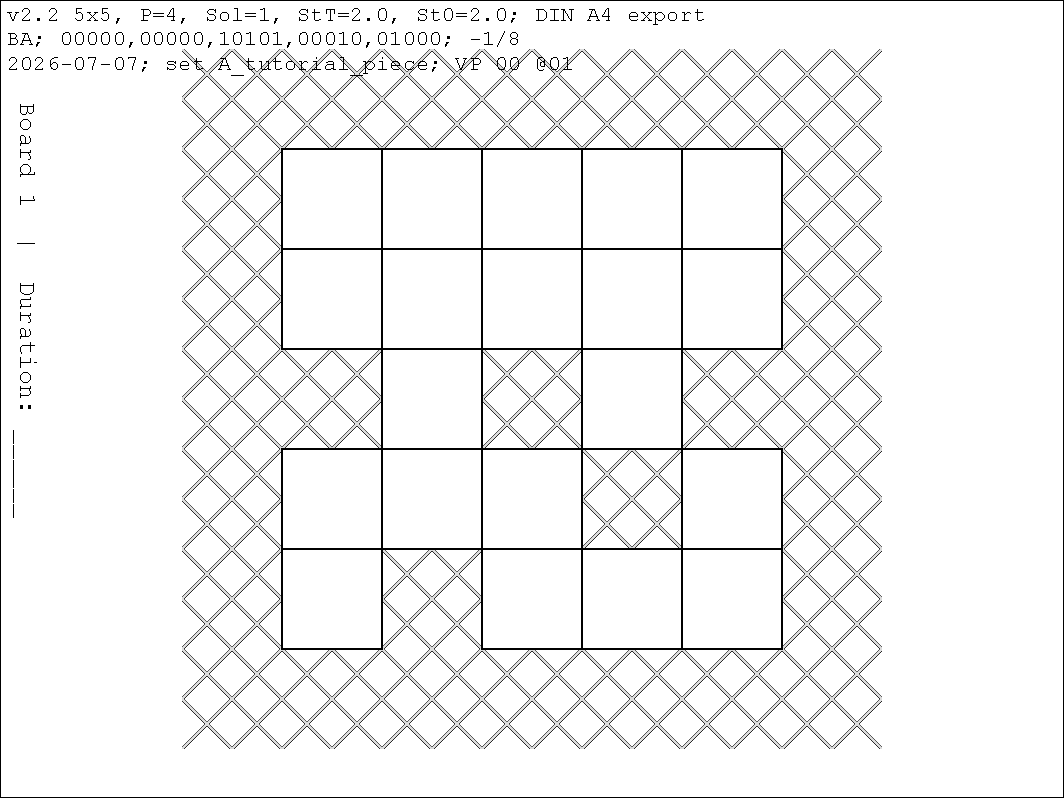
\includegraphics[
	angle=90,
	width=\paperwidth,
	height=\paperheight,
	keepaspectratio
	]{TutorialBoards/piece/dina4 01.png}%
}
\restoregeometry

{\tiny
L\"osungshinweise: \\
1. Nur eine Option um Zelle des U zu belegen \\
2. Analog N \\
3. U nicht doppelt erzwingt L \\
}




\FloatBarrier
\newpage
\subsection{Teilbarkeit der Zellanzahl durch 5}

Ein weiterer Trick:
Die Zellanzahl jedes abgeschlossenen Bereichs muss ein Vielfaches von 5 sein.
Grund:
Jeder Spielstein bedeckt genau 5 Zellen.
Ein Bereich mit z.\,B. 8 Zellen kann nicht gefüllt werden:
Ein Spielstein reicht nicht, und zwei passen nicht hinein.

\begin{figure}[hbt]
\centering
\tikzBoard{"60 techniques/divisibility by 5 example"}
\caption
{
Die gezeigte Platzierung von \piece{V} erzeugt zwei abgeschlossene Bereiche.
Links liegen 14 Zellen.
14 ist nicht durch 5 teilbar.
Eine Lösung ist daher unmöglich.
Diese Platzierung war falsch.
}
\end{figure}





\FloatBarrier
\subsection{Brett aufteilen}

Die Teilbarkeitsregel hilft, ein Brett in getrennte Bereiche zu teilen.
Diese Bereiche können dann einzeln gelöst werden.
Achte darauf, nicht den gleichen Spielstein in beiden Bereichen verwenden zu wollen.

\begin{figure}[hbt]
\centering
\tikzBoard{"60 techniques/board split example 1"}
\caption
{
Die Trennung entlang der Grenze zwischen Blau und Grün ist erzwungen.
Läge ein Spielstein in beiden Bereichen, wären die Zellzahlen dort nicht durch 5 teilbar.
}
\end{figure}



\newgeometry{margin=0pt}
%\thispagestyle{empty}
\noindent
\makebox[\paperwidth][c]{%
	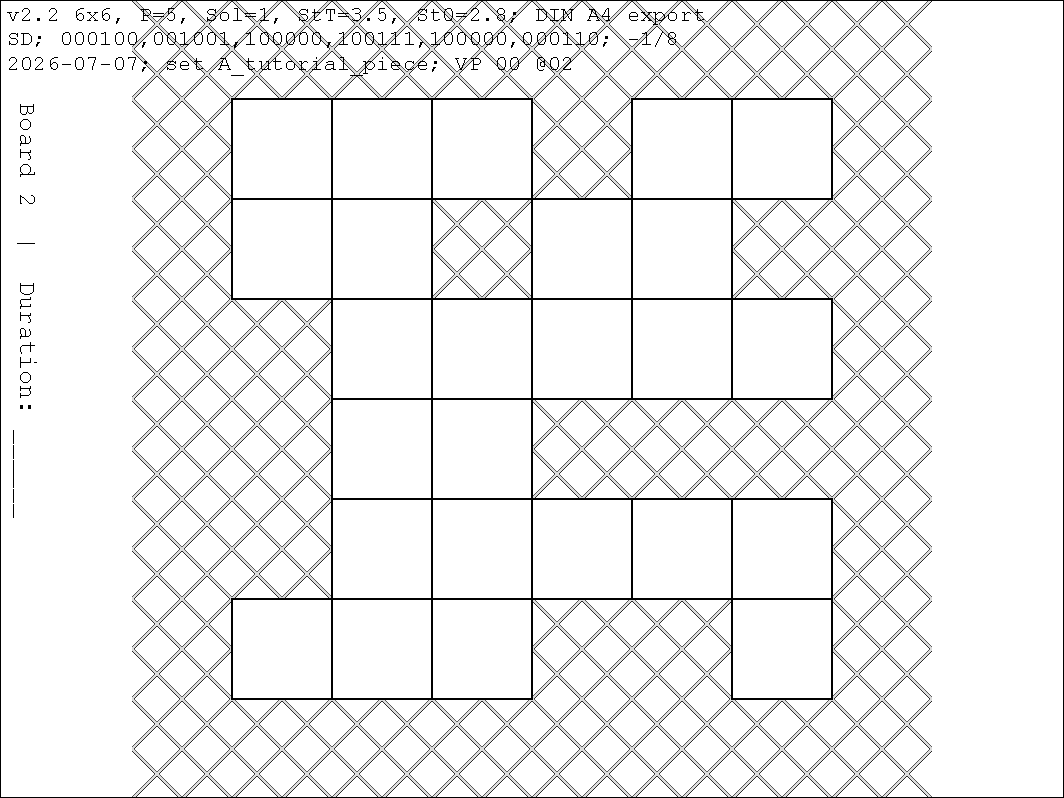
\includegraphics[
	angle=90,
	width=\paperwidth,
	height=\paperheight,
	keepaspectratio
	]{TutorialBoards/piece/dina4 02.png}%
}
\restoregeometry

{\tiny
L\"osungshinweise: \\
1. P, L erzwungen \\
2. T erzwungen \\
3. Y Konflikt erzwingt F \\
}


\newgeometry{margin=0pt}
%\thispagestyle{empty}
\noindent
\makebox[\paperwidth][c]{%
	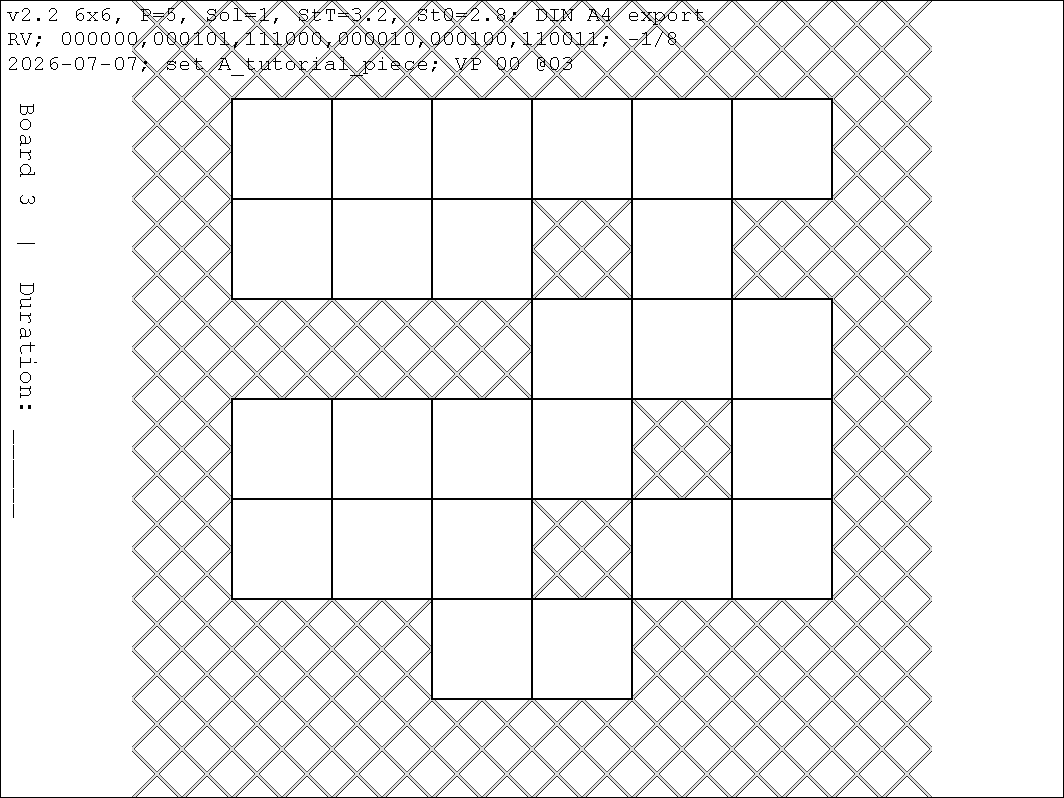
\includegraphics[
	angle=90,
	width=\paperwidth,
	height=\paperheight,
	keepaspectratio
	]{TutorialBoards/piece/dina4 03.png}%
}
\restoregeometry

{\tiny
L\"osungshinweise: \\
1. U, folgt Y, und P \\
2. U/N unmoeglich, muessen nebenlaufen \\
}


\newgeometry{margin=0pt}
%\thispagestyle{empty}
\noindent
\makebox[\paperwidth][c]{%
	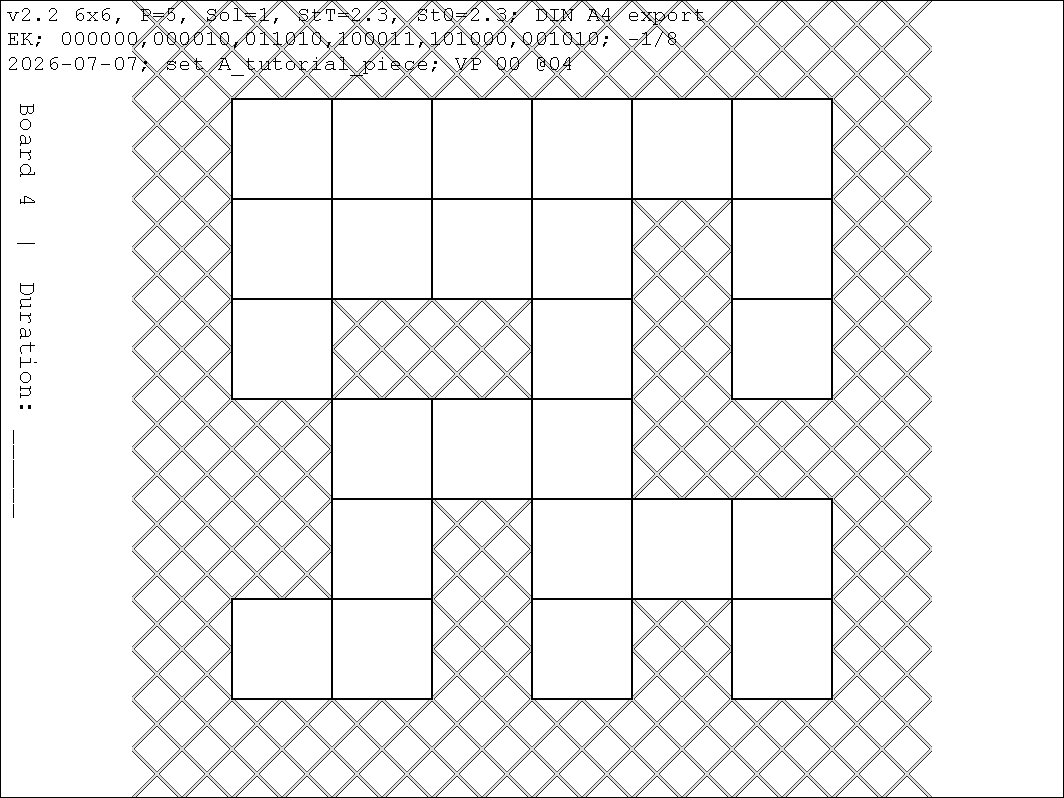
\includegraphics[
	angle=90,
	width=\paperwidth,
	height=\paperheight,
	keepaspectratio
	]{TutorialBoards/piece/dina4 04.png}%
}
\restoregeometry

{\tiny
Eigenstaendig loesen lassen. \\
L\"osungshinweise: \\
1. U, Z, V \\
2. N erzwungen \\
}


\newgeometry{margin=0pt}
%\thispagestyle{empty}
\noindent
\makebox[\paperwidth][c]{%
	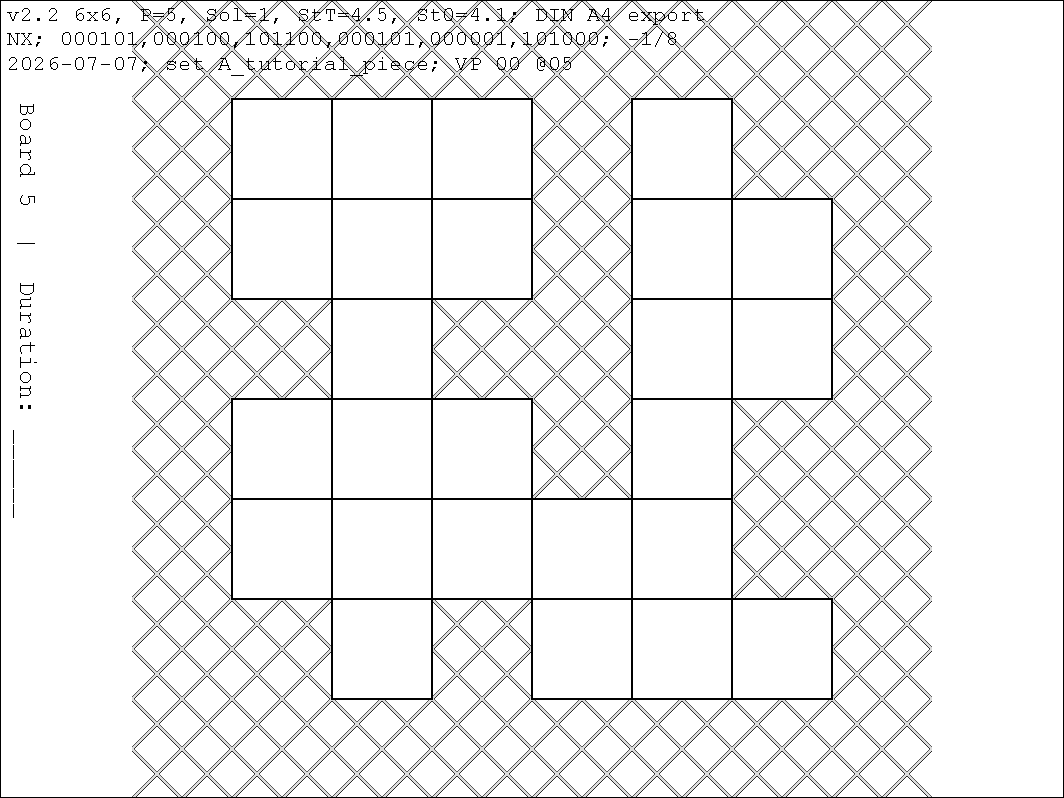
\includegraphics[
	angle=90,
	width=\paperwidth,
	height=\paperheight,
	keepaspectratio
	]{TutorialBoards/piece/dina4 05.png}%
}
\restoregeometry

{\tiny
L\"osungshinweise: \\
1. P \\
2. Erkenne T (wichtig!!!) \\
3. Erkenne U (wichtig!!!) \\
4. Jeder will zuerst T legen, geht aber nicht \\
}


\newgeometry{margin=0pt}
%\thispagestyle{empty}
\noindent
\makebox[\paperwidth][c]{%
	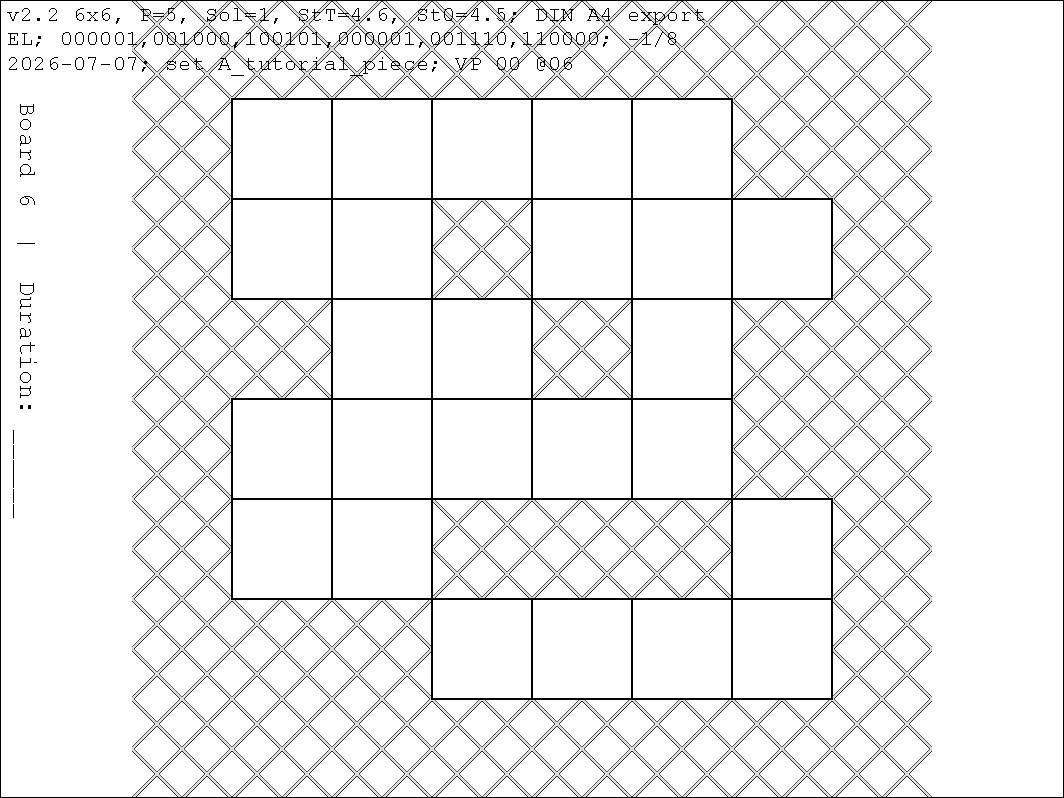
\includegraphics[
	angle=90,
	width=\paperwidth,
	height=\paperheight,
	keepaspectratio
	]{TutorialBoards/piece/dina4 06.png}%
}
\restoregeometry

{\tiny
L\"osungshinweise: \\
1. L \\
2. P erzwungen (wichtig!!!) \\
3. P Ausrichtung: erkenne Konflikt \\
4. Folgere W, Z \\
}


\newgeometry{margin=0pt}
%\thispagestyle{empty}
\noindent
\makebox[\paperwidth][c]{%
	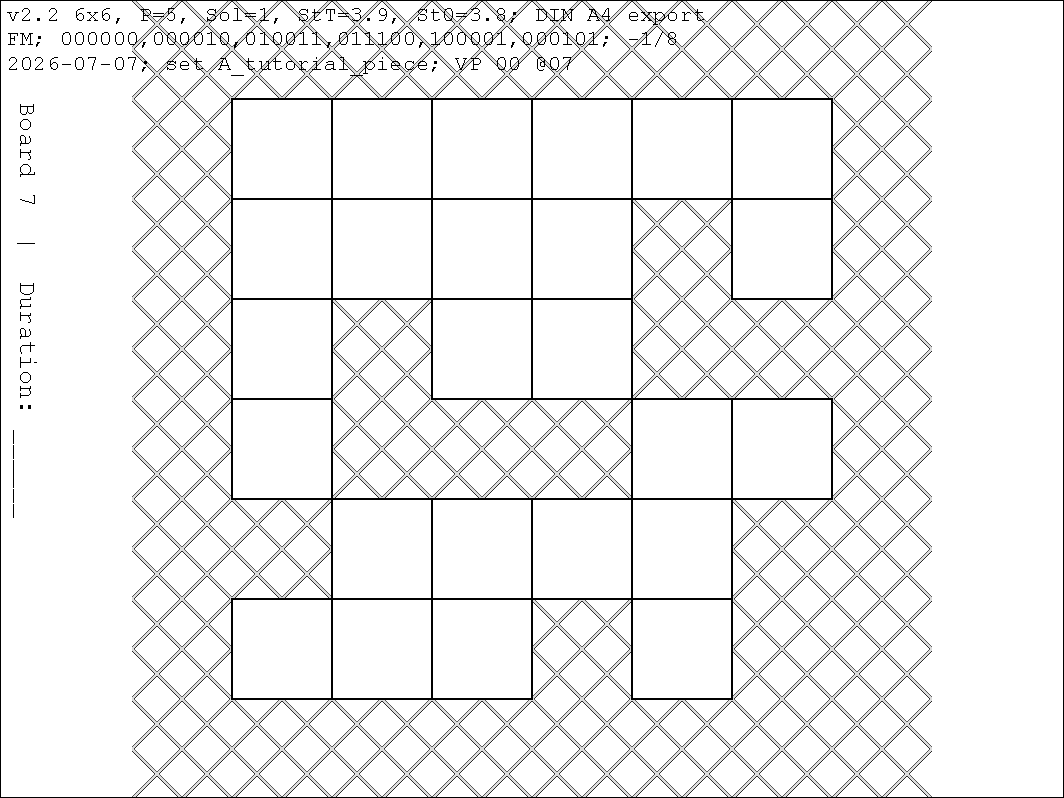
\includegraphics[
	angle=90,
	width=\paperwidth,
	height=\paperheight,
	keepaspectratio
	]{TutorialBoards/piece/dina4 07.png}%
}
\restoregeometry

{\tiny
Eigenstaendig loesen lassen. \\
L\"osungshinweise: \\
1. P, F \\
2. Groesste Einschraenkung ist U/L \\
3. Erkenne L erzwingt P = Konflikt \\
4. Folgere U \\
}





\FloatBarrier
\newpage
\subsection{Punktsymmetrische 10-Zellen-Bereiche}

Ein abgeschlossener Bereich mit genau 10 Zellen und Punktsymmetrie hat keine Lösung.
Das kommt selten vor, spart dann aber viel Arbeit.

Wichtig:
Der Bereich muss punktsymmetrisch sein,
also bei Drehung um 180 Grad um sein Zentrum gleich bleiben.
Achsensymmetrie reicht nicht.

\begin{figure}[hbt]
\centering
\begin{subfigure}[t]{0.30\linewidth}
\centering
\tikzBoard{"60 techniques/point symmetric 3"}
\caption{
Kein Paar verschiedener Spielsteine kann diesen punktsymmetrischen 10-Zellen-Bereich füllen.
}
\end{subfigure}
%
\hspace{0.03\linewidth}
%
\begin{subfigure}[t]{0.30\linewidth}
\centering
\tikzBoard{"60 techniques/point symmetric 2"}
\caption{
Dieser Bereich ist achsensymmetrisch und punktsymmetrisch.
Er ist daher nicht lösbar.
}
\end{subfigure}
%
\hspace{0.03\linewidth}
%
\begin{subfigure}[t]{0.30\linewidth}
\centering
\tikzBoard{"60 techniques/mirror symmetric 4"}
\caption{
Dieser Bereich ist nur achsensymmetrisch, aber nicht punktsymmetrisch.
Er ist mit \piece{F} und \piece{W} lösbar.
}
\end{subfigure}

\caption
{
}
\end{figure}






\FloatBarrier
\newpage
\section{Lösen mit Strängen}

Neue Idee:
Nicht direkt mit ganzen Spielsteinen arbeiten.
Stattdessen betrachtet man, welche benachbarten Zellen zum selben Spielstein gehören.
Solche Zellgruppen nennen wir \emph{Stränge}.
Ein Strang mit 5 Zellen entspricht einem Spielstein.
Wenn alle Zellen zu solchen 5er-Gruppen gehören
und kein Spielstein doppelt benutzt wird,
ist das Brett gelöst.

\begin{figure}[hbt]
\centering

\begin{subfigure}[t]{0.30\linewidth}
\centering
\tikzBoard{"40 string idea/string-intro-1"}
\caption{
Leeres Startbrett aus zehn Strängen.
Jeder Strang ist bisher nur eine einzelne Zelle.
}
\end{subfigure}
%
\hspace{0.03\linewidth}
%
\begin{subfigure}[t]{0.30\linewidth}
\centering
\tikzBoard{"40 string idea/string-intro-2"}
\caption{
Teillösung.
Stränge \str{3} und \str{8} wurden zu einem grö{\ss}eren Strang verbunden (grün).
Auch \str{2}, \str{6} und \str{7} wurden verbunden (blau).
}
\end{subfigure}
%
\hspace{0.03\linewidth}
%
\begin{subfigure}[t]{0.30\linewidth}
\centering
\tikzBoard{"40 string idea/string-intro-3"}
\caption{
Fertige Lösung.
Die beiden vorigen Stränge wurden vervollständigt:
Sie bestehen nun aus je fünf Zellen: \piece{P} und \piece{F}.
}
\end{subfigure}

\caption
[Feinschrittiger Fortschritt beim Lösen mit Strängen]
{
%Progress in string-based solving.
}
\label{fig:string-intro-1}
\end{figure}



\FloatBarrier
\newpage
\subsection{Teilweises Lösen}
Anders als ganze Spielsteine erlauben Stränge Teilergebnisse.
Engstellen lassen sich dabei gut nutzen.

\begin{figure}[hbt]
\centering

\begin{subfigure}[t]{0.3\linewidth}
\centering
\tikzBoard{"60 techniques/dead end small"}
\caption{
Die blaue Zelle dient als Engstelle.
So entsteht ein Strang aus drei Zellen.
Solche Sackgassen kommen häufig vor.
}
\label{fig:techniques/dead-end-small}
\end{subfigure}
%
\hspace{0.03\linewidth}
%
\begin{subfigure}[t]{0.3\linewidth}
\centering
\tikzBoard{"60 techniques/P piece"}
\caption{
Die blaue Engstelle trennt einen $2\times2$-Block in der Ecke ab.
Später müssen die vier Zellen Teil eines \piece{P} sein.
Die Ausrichtung ist noch offen.
}
\label{fig:techniques/p-piece}
\end{subfigure}
%
\hspace{0.03\linewidth}
%
\begin{subfigure}[t]{0.3\linewidth}
\centering
\tikzBoard{"60 techniques/dead end large"}
\caption{
Mit der blauen Engstelle entsteht ein \piece{U}.
Die Engstelle selbst gehört nicht zur gebildeten Gruppe.
}
\label{fig:techniques/dead-end-large}
\end{subfigure}

\caption
[Häufige Engstellenformen]
{
%Some of the more common bottleneck shapes.
}

\end{figure}




\FloatBarrier
Stränge erhöhen die Aussagekraft:
Man kann sagen, dass bestimmte Zellen zum selben Spielstein gehören müssen,
ohne schon zu wissen, welcher Spielstein es wird bzw. wie er ausgerichtet ist.

\begin{figure}[h]
\centering

\tikzBoard{"40 string idea/string based idea 2"}

\caption{
In diesem Beispiel ist bereits klar:
In der Ecke liegt ein \piece{P}, blau markiert.
Seine Ausrichtung ist noch offen.
Es wächst entweder nach rechts oder nach unten.
Das hängt allein davon ab, ob die vier Zellen in der geraden Linie ein \piece{I} oder ein \piece{L} bilden.
Das wiederum kann von anderen Brettbereichen abhängen.
}
\label{fig:string-approach-idea2}
\end{figure}


\FloatBarrier
Hinweis:
Die ganzen Tricks vom Lösens mit ganzen Spielsteinen gelten auch beim Lösen mit Strängen!
Die Teilbarkeit-durch-5-Regel,
die Brettaufteilung
und die Unlösbarkeit abgeschlossener punktsymmetrischer 10-Zellen-Bereiche sind weiterhin nützlich.

\newgeometry{margin=0pt}
%\thispagestyle{empty}
\noindent
\makebox[\paperwidth][c]{%
  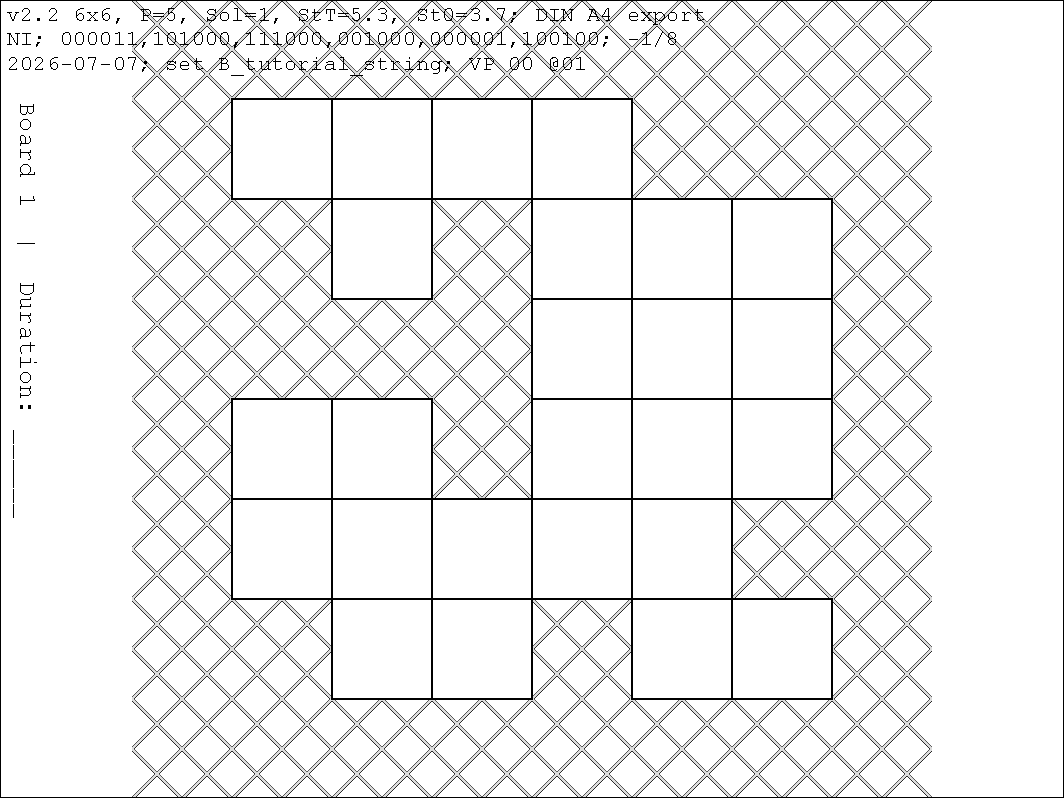
\includegraphics[
    angle=90,
    width=\paperwidth,
    height=\paperheight,
    keepaspectratio
  ]{TutorialBoards/01_easy}%
}
\restoregeometry

{\tiny
L\"osungshinweise: \\
1. Y per Abtrennung \\
2. P hat zwei Optionen, eine falsch \\
3. Zwei 3er Strings k\"onnen nicht verbunden werden \\
}


\FloatBarrier
\subsection{Stränge trennen, binäre Annahmen}

Ob zwei Zellen zum selben Spielstein gehören, ist binär:
wahr oder falsch.
Man kann annehmen, dass zwei Stränge nicht zum selben Spielstein gehören,
also \emph{getrennt} sind.
Das Trennen von Strängen führt oft schnell zu vielen Folgen.
Das ist gut:
Es gibt zwar viele Schritte,
aber jeder Schritt ist einfach.
Man kann gut vorausdenken.
Man sollte mit einem Zellpaar in einem eingeschränkten Bereich beginnen.

\begin{figure}[hbt]
\centering

\begin{subfigure}[t]{0.45\linewidth}
\centering
\tikzBoard{"40 string idea/easy to solve with split"}
\caption{
Die anfängliche Trennung (roter Balken) an einer guten Stelle erzeugt zwei Stränge.
Jeder hat nur einen einzigen Nachbarn zum Verbinden.
}
\end{subfigure}
\hspace{0.01\textwidth}
\begin{subfigure}[t]{0.45\linewidth}
\centering
\tikzBoard{"40 string idea/easy to solve with split step 1"}
\caption{
Nachdem beide gewachsen sind, können sie weiterhin nur nach links wachsen.
Sie müssen nebeneinander weiterlaufen.
}
\end{subfigure}
\hspace{0.01\textwidth}
\begin{subfigure}[t]{0.45\linewidth}
\centering
\tikzBoard{"40 string idea/easy to solve with split step 2"}
\caption{
Jetzt hat der grüne Strang keine sofort erzwungene Fortsetzung.
Der blaue Strang schon, und wird zwangsläufig zu \piece{V}.
}
\end{subfigure}
\hspace{0.01\textwidth}
\begin{subfigure}[t]{0.45\linewidth}
\centering
\tikzBoard{"40 string idea/easy to solve with split solved"}
\caption{
Der Rest des Bretts folgt schnell durch erzwungene Verbindungen an Engstellen.
}
\end{subfigure}

\caption
[Beispielbrett, das mit einer guten Trennung leicht lösbar ist]
{
Dieses Brett wird trivial lösbar, wenn man mit der Trennung der blau und grün markierten Stränge beginnt.
Danach gibt es keine weiteren Entscheidungen.
Jeder Schritt nach dem ersten ist erzwungen.
}
\label{fig:easy-to-solve-with-split}
\end{figure}

\FloatBarrier
\newpage


\newgeometry{margin=0pt}
%\thispagestyle{empty}
\noindent
\makebox[\paperwidth][c]{%
  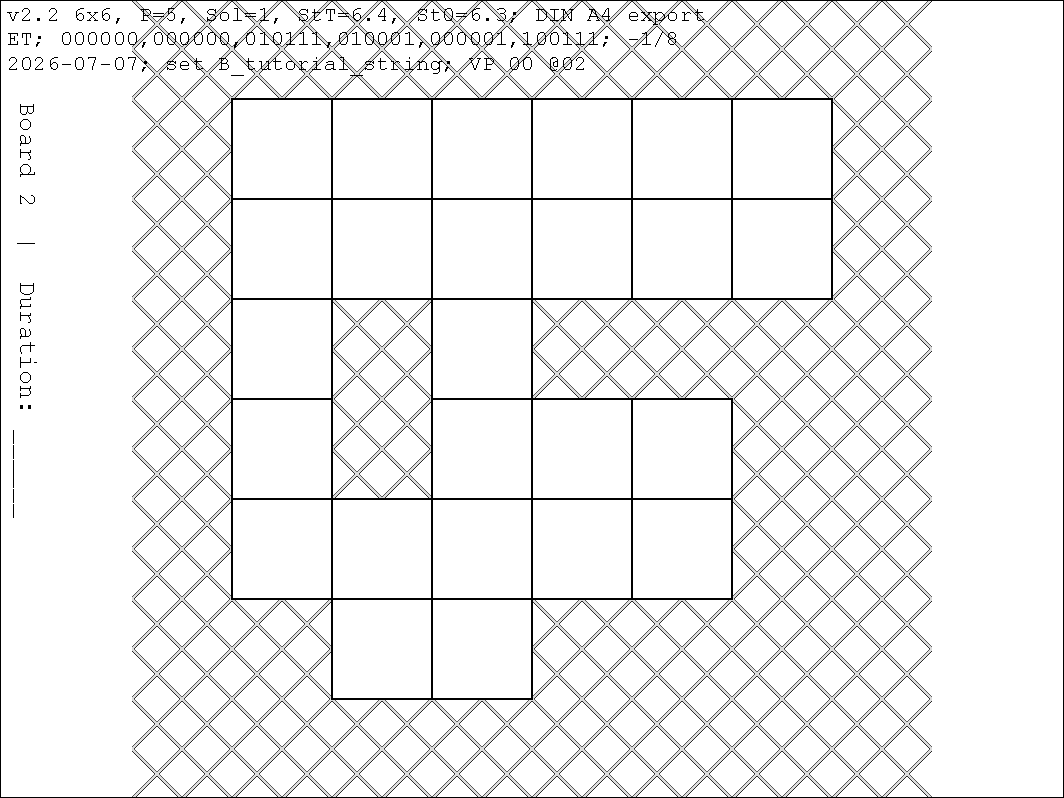
\includegraphics[
    angle=90,
    width=\paperwidth,
    height=\paperheight,
    keepaspectratio
  ]{TutorialBoards/02_easy_with_split}%
}
\restoregeometry


Wenn die Annahme einer Trennung in eine Sackgasse führt,
also zu einem unlösbaren Brett,
kann man das Ergebnis trotzdem nutzen:
Mit der Annahme gibt es keine Lösung.
Also gilt das Gegenteil:
Die Stränge gehören tatsächlich zum selben Spielstein und müssen verbunden werden.
Das folgt aus der binären Natur der Entscheidung.
Nutze diese Eigenschaft:
Stelle Annahmen auf,
widerlege sie,
und wende dann das Gegenteil an.

\begin{figure}[hbt]
\centering

\begin{subfigure}[t]{0.48\linewidth}
\centering
\tikzBoard{"40 string idea/wrong assumption 1"}
\caption{
Man könnte oben rechts beginnen.
Das ist sinnvoll, denn dort liegt ein enger Korridor.
Wir testen die Annahme:
Die blaue und die grüne Zelle sind getrennt.
}
\end{subfigure}
\hspace{0.01\textwidth}
\begin{subfigure}[t]{0.48\linewidth}
\centering
\tikzBoard{"40 string idea/wrong assumption 2"}
\caption{
Beide Stränge wachsen und laufen nebeneinander.
Der blaue Strang muss zu \piece{I} werden.
Da \piece{I} benutzt ist, muss der grüne Strang danach zu \piece{L} werden.
}
\end{subfigure}
\hspace{0.01\textwidth}
\begin{subfigure}[t]{0.48\linewidth}
\centering
\tikzBoard{"40 string idea/wrong assumption 4"}
\caption{
Dadurch entsteht unten eine Engstelle, die nur mit \piece{P} gefüllt werden kann (braun).
Das erzeugt direkt die nächste Engstelle und würde ein zweites \piece{P} benötigen (rot).
}
\end{subfigure}
\hspace{0.01\textwidth}
\begin{subfigure}[t]{0.48\linewidth}
\centering
\tikzBoard{"40 string idea/wrong assumption 5"}
\caption{
Einen Spielstein zweimal zu benutzen ist verboten.
Die Anfangsannahme war also falsch.
Die beiden Anfangszellen müssen zum selben Spielstein gehören und werden verbunden.
}
\end{subfigure}

\caption
[Beispielbrett, bei dem die Anfangstrennung verworfen wird und zu einer Verbindung führt]
{
In diesem Beispiel wählt der Spieler eine sinnvolle (aber nicht optimale) Stelle für die erste Trennungsannahme.
Zum Glück wird die Annahme auch bereits nach wenigen Schritten verworfen.
Durch die daraus folgende Verbindung entsteht Fortschritt.
}
\label{fig:merge-by-rejected-split}
\end{figure}


\FloatBarrier
\newgeometry{margin=0pt}
%\thispagestyle{empty}
\noindent
\makebox[\paperwidth][c]{%
  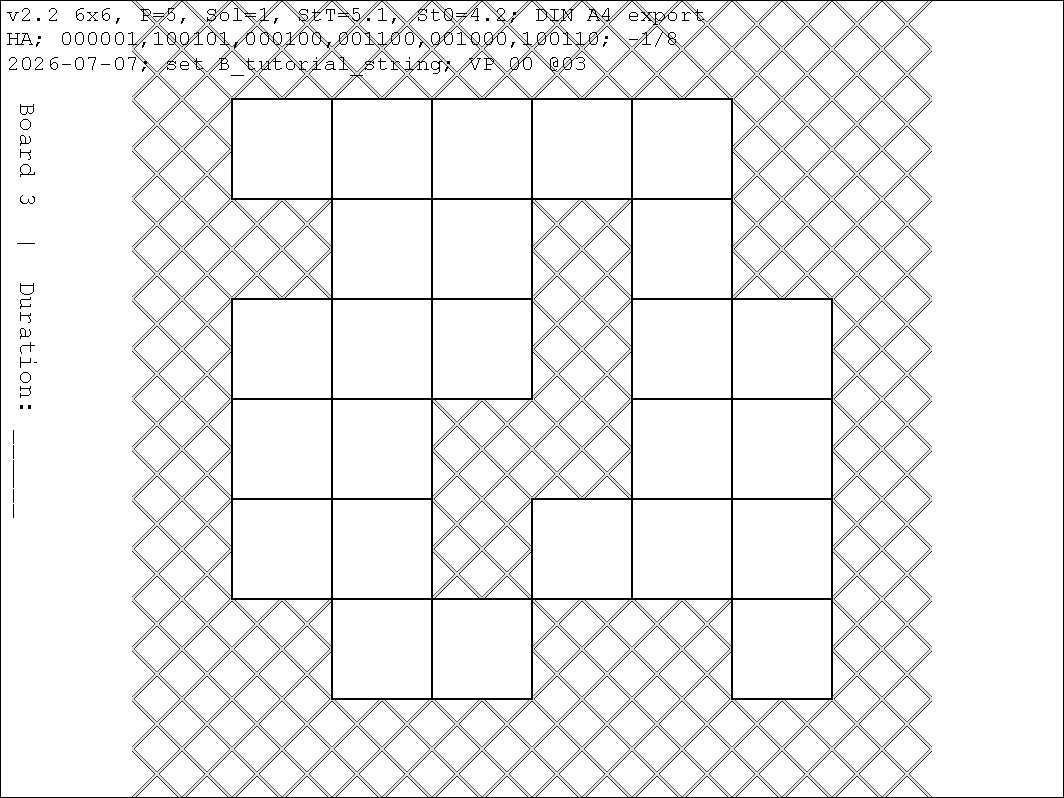
\includegraphics[
    angle=90,
    width=\paperwidth,
    height=\paperheight,
    keepaspectratio
  ]{TutorialBoards/03_easy_with_assumptions}%
}
\restoregeometry


{\tiny
L\"osungshinweise: \\
1. Unterteilung des Bretts \\
2. Im unteren Bereich, pr\"ufe Verbindung von den zwei 2er Strings und finde Kollision \\
3. Erzwingt Y in unbekannter Orientierung \\
4. Im oberen Bereich dann kein Y, nur N m\"oglich \\
5. Mittels Trennung von 3 vs 1 = Kollision unteren Bereich fertigstellen \\
}


\iffalse
\FloatBarrier
\subsection{Gegenseitig ausschlie{\ss}ende Verbindungen}

Wenn ein Strang fast fertig ist,
gibt es eine kleine Abkürzung im Denken.

\begin{figure}[hbt]
\centering

\tikzBoard{"40 string idea/choice 3plus2"}

\caption
{
Der blaue mittlere Strang aus 3 Zellen hat zwei einander ausschlie{\ss}ende Möglichkeiten zu wachsen.
Er kann sich links mit dem grünen Strang verbinden (Grö{\ss}e 2) und wäre dann fertig.
Oder er kann sich rechts mit dem braunen Strang verbinden (Grö{\ss}e 1).
Wegen der Grenze von 5 Zellen schlie{\ss}en sich diese Optionen gegenseitig aus.
}
\label{fig:string-choice-3plus2}
\end{figure}
\fi


\FloatBarrier
\subsection{Absichtliche Falschannahmen}

Suche aktiv nach Annahmen, die du widerlegen kannst.
Beispiel:
Wenn du wei{\ss}t, dass \piece{P} irgendwo auf dem Brett benutzt wird,
kannst du eine Annahme machen (verbinden oder trennen),
durch die ein weiteres \piece{P} benötigt werden würde?
Dann kannst du direkt das Gegenteil der Annahme als Tatsache vermerken und machst so Fortschritt.


\FloatBarrier
\newpage

Nach Wichtigkeit:
\\
\begin{tblr}{
colspec={Q[c,m]  Q[c,m]  X[m]},
colsep=2mm,
rowsep=5mm,
}

\textbf{1.}
&

\includegraphics[height=12mm, valign=c]{"img/60 techniques/P piece.png"}
&
{\textbf{Suche Engstellen und erzwungene Züge.}
\\-- Hat eine Zelle nur einen gültigen Nachbarn, ist die Verbindung erzwungen.
\\-- Erzwingt Teilbarkeit durch 5 eine Aufteilung des Bretts?
}\\

\textbf{2.}
&

\includegraphics[height=8mm, trim=50px 60px 0px 0px, clip, valign=c]{"img/40 string idea/wrong assumption 1.png"}
&
{\textbf{Bevorzuge enge Bereiche statt offener Flächen.}
Enge Korridore sind gut, besonders ihre Enden.
Je weniger Platz vorhanden ist, desto schneller entstehen Ergebnisse.
}\\

\textbf{3.}
&

\includegraphics[height=15mm, valign=c]{"img/40 string idea/wrong assumption 4.png"}
&
{\textbf{Trennen ist die Standardannahme.}
Es führt oft zu vielen Folgeschritten.
Entweder
a) das Brett wird gelöst,
oder b) das Brett wird unlösbar.
Im letzteren Fall ist das Gegenteil erzwungen: Sträge verbinden.
Trenne am besten in 2 Zellen breiten Korridoren,
damit zwei Stränge nebeneinander laufen müssen.
Wenn sich nicht schnell irgendetwas ergibt:
anderes Paar probieren.
}\\

\textbf{4.}
&

\includegraphics[height=12mm, trim=0px 0px 12px 25px, clip, valign=c]{"img/40 string idea/wrong assumption B 2.png"}
&
{\textbf{Arbeite in einem Bereich weiter, solange es Fortschritt gibt.}
Bleibe möglichst bei einem Bereich, bis er fertig ist.
Siehst du dort aber keine gute Fortsetzung mehr,
schau dir eine andere Stelle an.
}\\

\textbf{5.}
&

\includegraphics[height=15mm, valign=c]{"img/40 string idea/wrong assumption B 4.png"}
&
{Im Zweifelsfall:
\textbf{arbeite an den grö{\ss}ten Strängen weiter}.
Ein fertiger Strang belegt,
dass ein Spielstein anderswo nicht mehr verfügbar ist.
}\\

\end{tblr}


\FloatBarrier
\vspace{2em}

Regelverstö{\ss}e, mit denen du Annahmen verwerfen kannst:
\\
\begin{tblr}{
colspec={Q[c] X[m]},
rowsep=4mm,
colsep=1mm,
}


\includegraphics[height=15mm, valign=c]{"img/60 techniques/divisibility by 5 example.png"}
&
{Abgeschlossener Bereich mit Zellanzahl, die nicht durch 5 teilbar ist
}\\


\includegraphics[height=12mm, trim=0px 0px 14px 36px, clip, valign=c]{"img/40 string idea/wrong assumption 4.png"}
&
{Doppelte Nutzung eines Spielsteins
}\\


\includegraphics[height=10mm, valign=c]{"img/60 techniques/point symmetric 3.png"}
&
{Punktsymmetrischer abgeschlossener Bereich mit 10 Zellen
}\\

\end{tblr}




{\tiny
Wenn die Zeit es erlaubt:
An dieser Stelle die vorigen Übungsbretter, die noch ohne Stränge gelöst wurden, einmal mit Strängen lösen.
Dabei insbesondere die Grundlagen wiederholen.
Erzwungene Sequenzen sollten schnell gefunden werden.
Man sollte auch zuverlässig gute (nicht unbedingt optimale) Fortsetzungspunkte wählen können.
Ziel ist es, rasch zwischen diesen wechseln zu können, sollten sie sich als kompliziert herausstellen.

Die hier nachfolgenden Bretter sind dann noch etwas schwerer.
}




\iffalse
\begin{figure}[hbt]
\centering

\begin{subfigure}[t]{0.48\linewidth}
\centering
\tikzBoard{"40 string idea/wrong assumption B 1"}
\caption{
Yet another attempt on this board.
This time, we start in the very bottom, which is perhaps not the most ideal spot.
The blue string quickly becomes a \piece{N} next.
}
\end{subfigure}
\hspace{0.01\textwidth}
\begin{subfigure}[t]{0.48\linewidth}
\centering
\tikzBoard{"40 string idea/wrong assumption B 2"}
\caption{
The green string is more tricky.
It cannot connect up, as this would leave 4 cells to its right, but at most 2 fit into the green string.
(Alternatively, some nested merge-split-decisions also quickly prove this.)
It must become a \piece{Z}.
}
\end{subfigure}
\hspace{0.01\textwidth}
\begin{subfigure}[t]{0.48\linewidth}
\centering
\tikzBoard{"40 string idea/wrong assumption B 4"}
\caption{
To finish this string, there are three mutually exclusive options.
Going left and becoming a \piece{Z} is illegal, because \piece{Z} is already used.
Going up into a \piece{L} would leave a closed-off area of 4 cells.
So going to the right into a \piece{U} is the only path we can try.
}
\end{subfigure}
\hspace{0.01\textwidth}
\begin{subfigure}[t]{0.48\linewidth}
\centering
\tikzBoard{"40 string idea/wrong assumption B 5"}
\caption{
However, this is also a dead end:
The double-\piece{P} strikes again.
We conclude that our initial assumption was wrong and the initial pair of cells should be merged.
}
\end{subfigure}

\caption
[Split 3 xxx]
{
Going at this board from the bottom leads to minor complications with the green string.
When these are resolved, the brown string can accept only 1 out of 3 options.
They all turn out to be dead ends, so we reject the assumption to make progress.
}
\label{fig:split3}
\end{figure}

\fi



%TODO examples

%\newpage
%\adjustbox{width = \textwidth}{
%\input{img/trees/v60/psylab 00; -1; divisibility, example/soltree string, e2.3 visits, e3.3 steps/tree img=1 write=[,,].tex}
%}



\FloatBarrier
\newgeometry{margin=0pt}
%\thispagestyle{empty}
\noindent
\makebox[\paperwidth][c]{%
  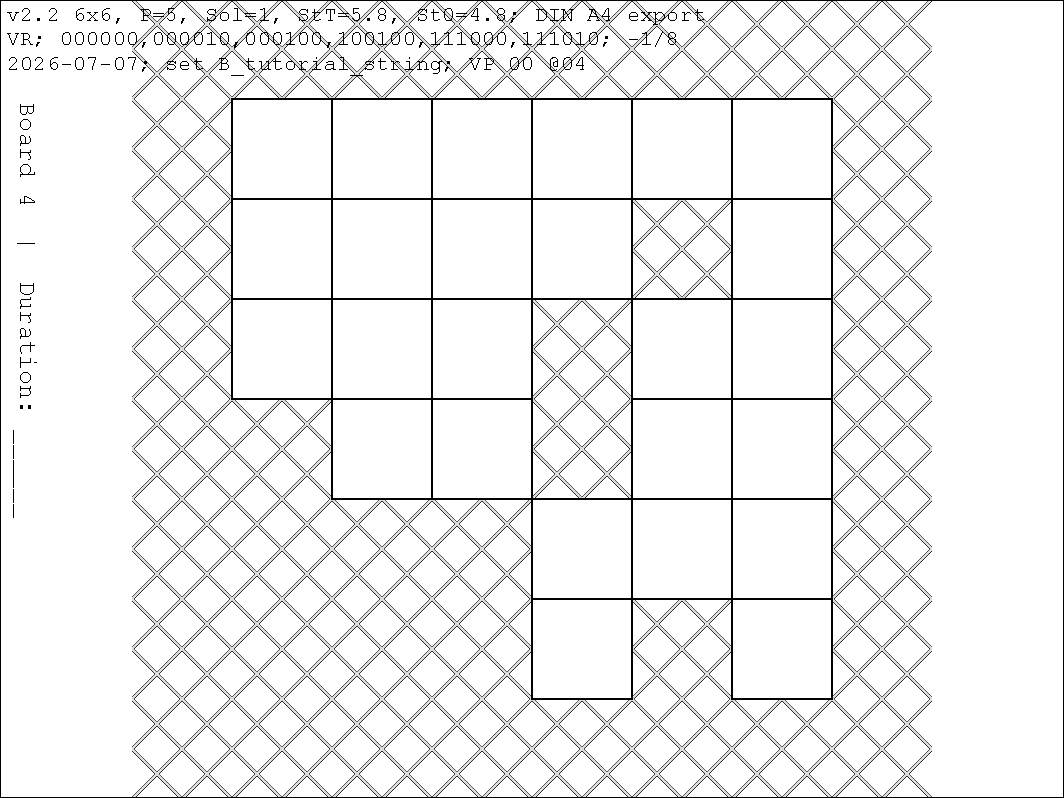
\includegraphics[
    angle=90,
    width=\paperwidth,
    height=\paperheight,
    keepaspectratio
  ]{TutorialBoards/04_hard_whole_board}%
}
\restoregeometry

{\tiny
L\"osungshinweise: \\
1. Unterteilung des Bretts \\
2. Im oberen Bereich erkenne Optionen I+N oder P+U \\
3. Im unteren Bereich finde 4 Optionen des 3er Strings: I, I, N, L \\
4. Eliminiere sofort L. Y auch wegen Punktsymmetrie. \\
5. Folgere oben P+U. \\
6. Beste Einschraenkung unten per N, Fehlschlag \\
7. Erzwingt I, Rest folgt \\
}



\FloatBarrier
\newgeometry{margin=0pt}
%\thispagestyle{empty}
\noindent
\makebox[\paperwidth][c]{%
  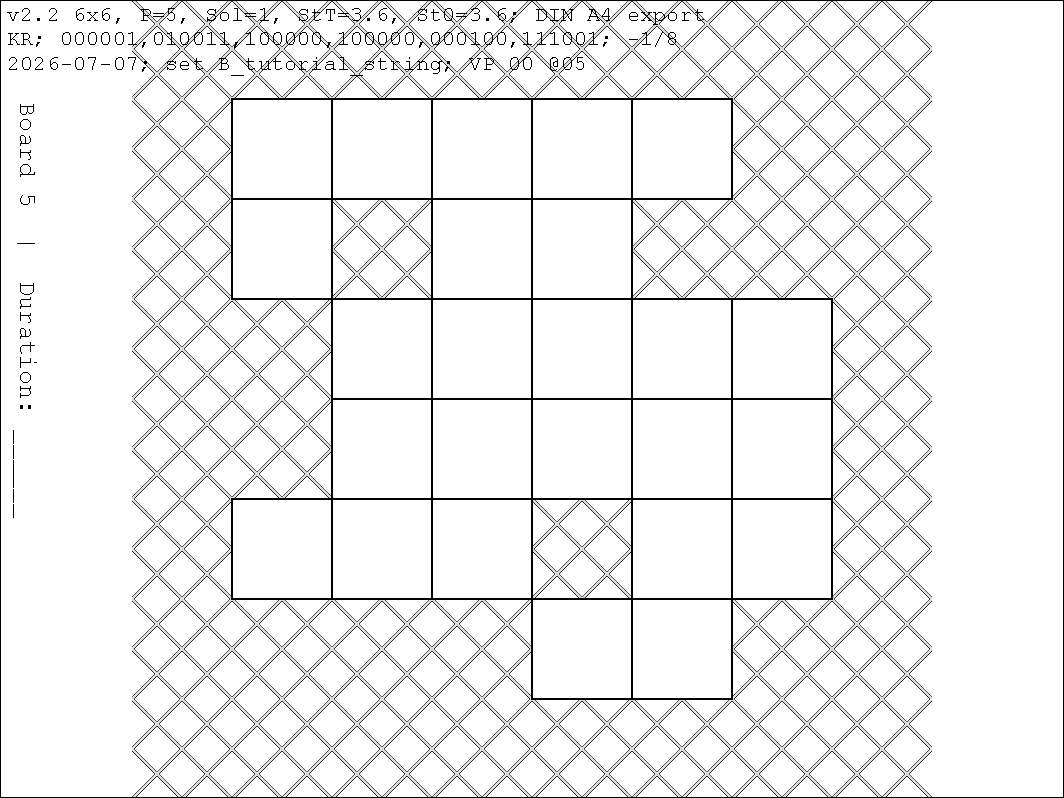
\includegraphics[
    angle=90,
    width=\paperwidth,
    height=\paperheight,
    keepaspectratio
  ]{TutorialBoards/05_test}%
}
\restoregeometry


{\tiny
Dieses Brett zur Verifikation nutzen. \\
L\"osungshinweise: \\
1. 2er + 4er muessen getrennt sein, erzwingt U. \\
2. Optionen L, U, Z; eliminiere U und L \\
3. Engstelle erzwingt T \\
4. 3er + 3er getrennt, Rest folgt \\
}


\end{document}
